% Use the following line _only_ if you're still using LaTeX 2.09.
%\documentstyle[icml2017,epsf,natbib]{article}
% If you rely on Latex2e packages, like most moden people use this:
\documentclass{article}

% use Times
\usepackage{times}
% For figures
\usepackage{graphicx} % more modern
%\usepackage{epsfig} % less modern
\usepackage{subfigure} 

% For citations
\usepackage[sort&compress]{natbib}

% For algorithms
\usepackage{algorithm}
\usepackage{algorithmic}
\usepackage{amsthm,amssymb,amsopn,amsmath}

% As of 2011, we use the hyperref package to produce hyperlinks in the
% resulting PDF.  If this breaks your system, please commend out the
% following usepackage line and replace \usepackage{icml2017} with
% \usepackage[nohyperref]{icml2017} above.
\usepackage{hyperref}

% Packages hyperref and algorithmic misbehave sometimes.  We can fix
% this with the following command.
\newcommand{\theHalgorithm}{\arabic{algorithm}}

% Employ the following version of the ``usepackage'' statement for
% submitting the draft version of the paper for review.  This will set
% the note in the first column to ``Under review.  Do not distribute.''
\usepackage{icml2017} 

% Employ this version of the ``usepackage'' statement after the paper has
% been accepted, when creating the final version.  This will set the
% note in the first column to ``Proceedings of the...''
%\usepackage[accepted]{icml2017}
\newtheorem{assumption}{Assumption}
\newtheorem{define}{Definition}
\newtheorem{thm}{Theorem}
\newtheorem{lem}{Lemma}
\newtheorem{coro}{Corollary}

% The \icmltitle you define below is probably too long as a header.
% Therefore, a short form for the running title is supplied here:
\icmltitlerunning{Counterfactual Fairness-- Suplementary Materials}

\begin{document} 

\twocolumn[
\icmltitle{Counterfactual Fairness -- Supplementary Materials}

% It is OKAY to include author information, even for blind
% submissions: the style file will automatically remove it for you
% unless you've provided the [accepted] option to the icml2017
% package.

% list of affiliations. the first argument should be a (short)
% identifier you will use later to specify author affiliations
% Academic affiliations should list Department, University, City, Region, Country
% Industry affiliations should list Company, City, Region, Country

% you can specify symbols, otherwise they are numbered in order
% ideally, you should not use this facility. affiliations will be numbered
% in order of appearance and this is the preferred way.
\icmlsetsymbol{equal}{}

\begin{icmlauthorlist}
\icmlauthor{Cieua Vvvvv}{goo}
%\icmlauthor{Iaesut Saoeu}{ed}
\end{icmlauthorlist}

\icmlaffiliation{goo}{Googol ShallowMind, New London, Michigan, USA}
\icmlaffiliation{ed}{University of Edenborrow, Edenborrow, United Kingdom}

\icmlcorrespondingauthor{Cieua Vvvvv}{c.vvvvv@googol.com}

% You may provide any keywords that you 
% find helpful for describing your paper; these are used to populate 
% the "keywords" metadata in the PDF but will not be shown in the document
\icmlkeywords{Causality,Counterfactual,Fairness}

\vskip 0.3in
]
\setcounter{section}{4}
% this must go after the closing bracket ] following \twocolumn[ ...

% This command actually creates the footnote in the first column
% listing the affiliations and the copyright notice.
% The command takes one argument, which is text to display at the start of the footnote.
% The \icmlEqualContribution command is standard text for equal contribution.
% Remove it (just {}) if you do not need this facility.

%\printAffiliationsAndNotice{}  % leave blank if no need to mention equal contribution
%\printAffiliationsAndNotice{\icmlEqualContribution} % otherwise use the standard text.
%\footnotetext{hi}
To satisfy space requirements section 5 of the original paper was condensed.
A longer version covering more ground with greater exposition is included here.
\section{Extended Methods and Assessment}
\setcounter{subsection}{1} 
Various design choices lead to the definition of $\hat Y$ and its fitting. Given a causal model, these choices include:% the following:

First, $\hat Y$ is a function of $U \cup X$ even though our notation emphasizes its dependence on $U$. This also means it can be a function of a subset of this set, and any element of $X$ which is not a descendant of $A$ can be used. If only a strict subset of $U$ is used, the causal model need not be fully specified: equation $V_i = f_i(pa_i, U_{pa_i})$ can be substituted by a non-deterministic conditional probability $p(V_i\ |\ pa_i, U_{pa_i}')$, where $U_{pa_i}' \subset U_{pa_i}$ and $p(V_i\ |\ pa_i, U_{pa_i}') = \int f_i(pa_i, U_{pa_i}) d U_{pa_i}''$, where $U_{pa_i}'' \equiv U_{pa_i} \backslash U_{pa_i}'$. This marginalization has implications in modeling discussed in the next section.

Second, any random variable generated independently is trivially counterfactually fair. It is tacitly understood that $\hat Y$ should be a {\it good} predictor, not something like tossing a coin. That is, $\hat Y$ is to be understood as a parameterized function $g_\theta(U, X)$ where $\theta$ is learned by minimizing (an empirical version of) the expected loss $E[l(Y, g_\theta(U, X))\ | X,
  A]$, where the expectation is over $A \cup X \cup U \cup \{Y\}$. For instance, $l(Y, g_\theta(U, X)) = (Y - g_\theta(U, X))^2$, or the log-loss for Bernoulli classification.  In practice, the distribution of $A \cup X \cup \{Y\}$ can be the empirical distribution as given by some training data, while $p(U\ |\ X, A)$ comes from the estimated causal model fit to the same training data. Markov chain Monte Carlo (MCMC) may be necessary to generate samples from this conditional, which means every training data point is replaced by a set of data points sharing the same $A \cup X \cup \{Y\}$ but with different replicates of $U$. Any predictor can be used as $g_\theta(U, X)$ including random forests and neural networks.
\subsection{Limitations and a Guide for Model Building}
Causal modeling requires untestable assumptions. Experimental data can sometimes be used to infer causal connections, but counterfactual modeling adds another layer of complexity by requiring functional decompositions between background and endogenous variables or, equivalently, joint distributions among variables which belong to separate physical realities. Such decompositions are in general not uniquely identifiable even with experimental data, which has motivated causal modeling frameworks that avoid counterfactuals entirely unless where they are strictly necessary \citep{dawid:00}. As in several matters of law and regulation, fairness at an individual level is a counterfactual quantity and some level of counterfactual assumptions are unavoidable. As a guide for building fair predictive models, we categorize assumptions by three levels of increasing strength.
%
\begin{itemize}
\item[L1] Given a causal DAG, build $\hat Y$
  using as covariates only the observable variables which are not
  descendants of the protected attributes $A$ in the DAG(s). This
  requires partial information about the causal DAG, but no
  assumptions about structural equations and priors over background
  variables. Within our definition (5), here
  $\hat Y$ cannot be a function of $U$ but is allowed to be a function
  of any subset of $X$ that is not a descendant of $A$;
\item[L2] The above might waste much information, particularly if the
  protected attributes are typical demographic information such as
  race, sex, gender and age, which can be parents but not children of
  other variables in the DAG. To include information from descendants
  of $A$, postulate background latent variables that act as latent
  causes of observable variables, based on explicit domain knowledge
  and learning algorithms with causal assumptions\footnote{In some
    domains, it is actually common to build a model entirely around
    latent constructs which have few or no observable parents nor
    connections among observed variables \citep{bol:89}.}.  As these
  (latent) variables are not descendants of $A$, they can be used.
  Conditioning on descendants of $A$ will propagate information from
  $X$ to them. The dependency of each $V_i$ on its parents can be
  probabilistic, instead of given by a structural equation, as
  explained in the previous section;
\item[L3] In the above construction, the model still factorizes as a
  general DAG model, where each node follows a non-degenerate
  distribution given observed and latent variables. In the final level
  of assumptions, remove all randomness from the conditional
  distributions to obtain a full decomposition $(U, V, F)$ of the
  model. Default assumptions, partially independent of the domain,
  might be invoked. For instance, we can model the conditional
  distribution $p(V_i\ |\ V_1, \dots, V_{i - 1})$ as an additive error
  model, $V_i = f_i(V_1, \dots, V_{i - 1}) + e_i$ \citep{peters:14}. The error
  term $e_i$, now assumed to be a summary of the other latent causes
  of $V_i$, then becomes an input to $\hat Y$ after conditioning on
  the observable variables. This maximizes the amount of information
  that can be properly extracted from a causal model by the fair
  predictor $\hat Y$.
\end{itemize}

\subsection{Testing assumptions}
There is already a wealth of literature on the topic of testing implications of modeling assumptions, with \citep{bollen:93} providing a classic account aimed at structural equation models. There are as well tools that help the (partial) discovery of causal structure \citep{sgs:00,peters:14} and latent variables \citep{silva:10b,HalpernSontag_uai13,anima:14}.

Our view is that fairness should be the consequence of clear assumptions that need to be defended given the extent of existing available evidence, but with the understanding that there will be a subset of assumptions which cannot be tested. The ultimate validation of a counterfactual model is a matter of agreement between regulators and algorithm designers, lying outside the realm of machine learning theory and within the subject matter of the domain. The goal of counterfactual fairness is to provide a foundation for justifying particular modeling choices, which otherwise may sound arbitrary. With counterfactual fairness, assumptions are laid out in the open for criticism by regulators and society.


\section{Details of NYPD experiment}

\begin{figure}[th]
\begin{center}
\vspace{-1ex}
\centerline{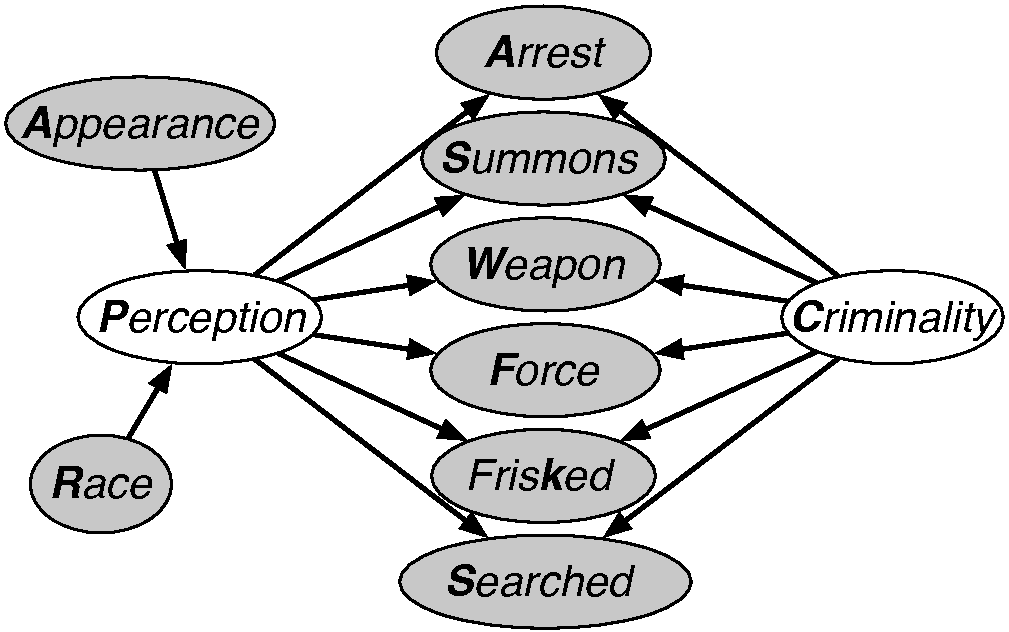
\includegraphics[width=\columnwidth]{stop_and_frisk_model3.pdf}}
\vspace{-2ex}
\caption{A causal model for the stop and frisk dataset.\label{figure.stop_and_frisk}\vspace{-4ex}}
\vspace{-2ex}
\end{center}
\end{figure}

\paragraph{Model.}
We model this stop-and-frisk data using the graph in Figure~\ref{figure.stop_and_frisk}. Specifically, we posit main causes for the observations: \emph{Arrest} (if an individual was arrested), \emph{Summons} (an individual was called to a court-summons), \emph{Weapon} (an individual was found to be carrying a weapon), \emph{Force} (some sort of force was used during the stop), \emph{Frisked}, and \emph{Searched}. The first cause of these observations is some measure of an individual's latent \emph{Criminality}, which we do not observe. We believe there is an additional cause, an individual's perceived criminality, \emph{Perception}, also unobserved. This second factor is introduced as we believe that these observations may be biased based on an officer's perception of whether an individual is likely a criminal or not. This perception is affected by an individual's \emph{Appearance} and their \emph{Race}. In this sense \emph{Criminality} is counterfactually fair, while \emph{Perception} models how race affects each of the other observed variables.

\paragraph{Criminality and perception distributions.}
After fitting this model to the data we can look at the distribution of \emph{Criminality} and \emph{Perception} across different races, shown as box plots in Figure~\ref{figure.stop_and_frisk}. We see that the median criminality for each race is nearly identical, while the distributions are somewhat different, demonstrating that \emph{Criminality} approaches demographic parity. The differences that due exist may be due to unobserved confounding variables that are affected by race or unmodeled noise in the data. On the right \emph{Perception} varies considerably by race with white individuals having the lowest perceived criminality while black and black Hispanic individuals have the highest.

\begin{figure}[!th]
\begin{center}
%\vspace{-1ex}
\centerline{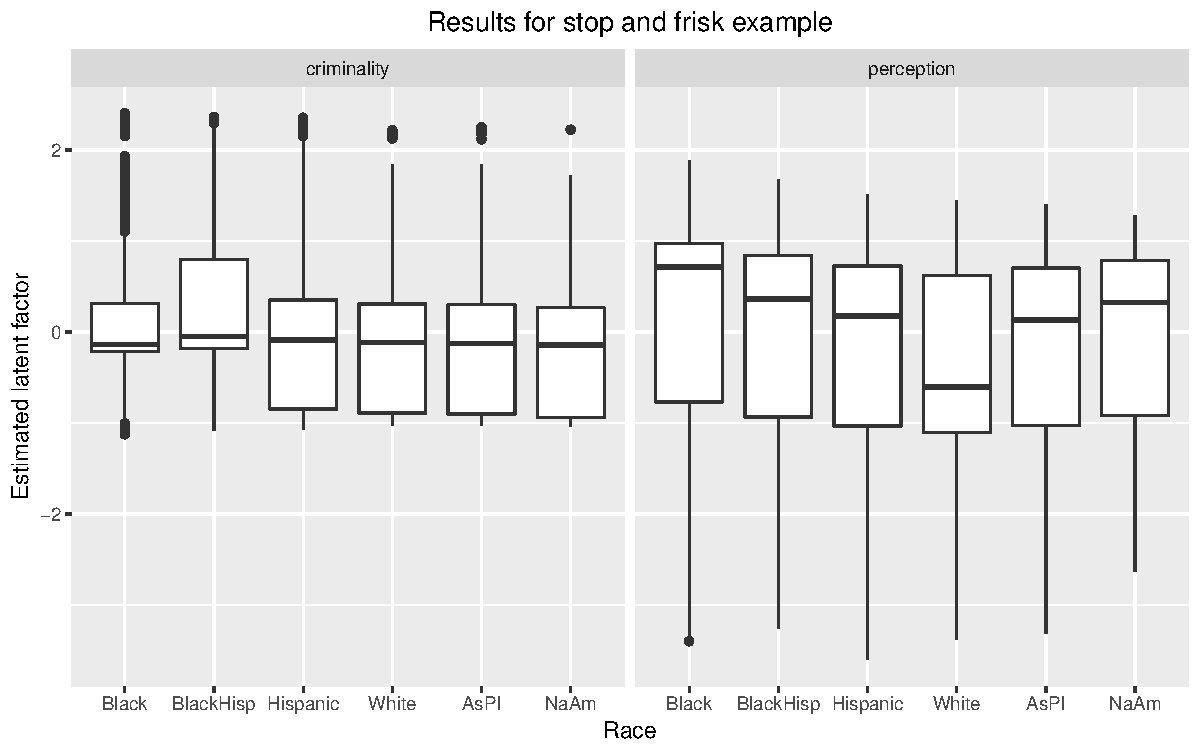
\includegraphics[width=\columnwidth]{stopandfrisk_output.pdf}}
\vspace{-2ex}
\caption{Distributions of estimated latent perception and criminality scores for the stop and frisk dataset.\label{figure.stop_and_frisk_output}\vspace{-5ex}}
\vspace{-2ex}
\end{center}
\end{figure}


\bibliography{rbas,bibliography}
\bibliographystyle{icml2017}

\end{document} 


% This document was modified from the file originally made available by
% Pat Langley and Andrea Danyluk for ICML-2K. This version was
% created by Lise Getoor and Tobias Scheffer, it was slightly modified  
% from the 2010 version by Thorsten Joachims & Johannes Fuernkranz, 
% slightly modified from the 2009 version by Kiri Wagstaff and 
% Sam Roweis's 2008 version, which is slightly modified from 
% Prasad Tadepalli's 2007 version which is a lightly 
% changed version of the previous year's version by Andrew Moore, 
% which was in turn edited from those of Kristian Kersting and 
% Codrina Lauth. Alex Smola contributed to the algorithmic style files.  

%%% Local Variables:
%%% mode: latex
%%% TeX-master: "ricardo_draft"
%%% End:
